\PassOptionsToPackage{dvipsnames,svgnames,x11names}{xcolor}
\documentclass[tikz,border=8pt]{standalone}
\usetikzlibrary{arrows.meta,positioning,calc,shapes,shadows,decorations.pathmorphing,shapes.geometric,backgrounds,decorations.markings,decorations.pathreplacing,decorations.text,fit,shapes.misc,shapes.arrows,matrix,bending,3d,chains,intersections,shapes.symbols,svg.path,shapes.multipart,snakes,shapes.callouts,angles,quotes}
\providecolor{gold}{RGB}{212,175,55}
\providecolor{silver}{RGB}{192,192,192}
\providecolor{bronze}{RGB}{205,127,50}
\providecolor{darkblue}{RGB}{0,0,139}
\providecolor{lightblue}{RGB}{173,216,230}
\providecolor{darkgreen}{RGB}{0,100,0}
\providecolor{lightgreen}{RGB}{144,238,144}
\providecolor{darkred}{RGB}{139,0,0}
\providecolor{navy}{RGB}{0,0,128}
\providecolor{skyblue}{RGB}{135,206,235}
\providecolor{beige}{RGB}{245,245,220}
\providecolor{cream}{RGB}{255,253,208}
\usepackage{amsmath}
\usepackage{amssymb}
\usepackage{fontawesome5}
\usetikzlibrary{fadings,shadows.blur,patterns,patterns.meta}

\usepackage{amsmath}
\usepackage{amssymb}
\usepackage{fontawesome5}
\usepackage{xcolor}

\providecolor{gold}{RGB}{212,175,55}
\providecolor{silver}{RGB}{192,192,192}
\providecolor{bronze}{RGB}{205,127,50}
\providecolor{darkblue}{RGB}{0,0,139}
\providecolor{lightblue}{RGB}{173,216,230}
\providecolor{darkgreen}{RGB}{0,100,0}
\providecolor{lightgreen}{RGB}{144,238,144}
\providecolor{darkred}{RGB}{139,0,0}
\providecolor{navy}{RGB}{0,0,128}
\providecolor{skyblue}{RGB}{135,206,235}
\providecolor{beige}{RGB}{245,245,220}
\providecolor{cream}{RGB}{255,253,208}

% --- Custom Color Palette ---
\definecolor{codebg}{RGB}{33, 37, 43}
\definecolor{codetext}{RGB}{230, 230, 230}
\definecolor{accentblue}{RGB}{0, 150, 255}
\definecolor{failred}{RGB}{220, 53, 69}
\definecolor{passgreen}{RGB}{40, 167, 69}
\definecolor{textdark}{RGB}{40, 40, 40}

% macOS Window Controls
\definecolor{macred}{RGB}{255, 95, 86}
\definecolor{macyellow}{RGB}{255, 189, 46}
\definecolor{macgreen}{RGB}{39, 201, 63}

% Syntax Highlighting Tokens
\definecolor{synTag}{RGB}{97, 175, 239}
\definecolor{synAttr}{RGB}{152, 195, 121}
\definecolor{synString}{RGB}{229, 192, 123}
\definecolor{synPunct}{RGB}{171, 178, 191}

\begin{document}
\begin{tikzpicture}[
    show background rectangle,
    background rectangle/.style={fill=white},
    % --- IDE Window Code Block Style ---
    idecard/.style={
        draw=black!75,
        line width=0.8pt,
        fill=codebg,
        text=codetext,
        rounded corners=6pt,
        blur shadow={shadow opacity=28, shadow yshift=-3pt, shadow blur radius=4pt},
        inner ysep=18pt,
        inner xsep=10pt,
        text width=7.8cm,
        minimum width=8.5cm,
        align=left,
        font=\ttfamily\small,
        path picture={
            % Top macOS header bar
            \fill[black!85] (path picture bounding box.north west) rectangle ([yshift=-13pt]path picture bounding box.north east);
            \draw[black!65, line width=0.4pt] ([yshift=-13pt]path picture bounding box.north west) -- ([yshift=-13pt]path picture bounding box.north east);
            % Window Dots
            \fill[macred] ([xshift=10pt, yshift=-6.5pt]path picture bounding box.north west) circle (2.2pt);
            \fill[macyellow] ([xshift=17pt, yshift=-6.5pt]path picture bounding box.north west) circle (2.2pt);
            \fill[macgreen] ([xshift=24pt, yshift=-6.5pt]path picture bounding box.north west) circle (2.2pt);
        }
    },
    % --- Glassmorphic Logic Evaluation Card Style (Fail) ---
    logiccard_fail/.style={
        fill=white,
        fill opacity=0.96,
        text opacity=1,
        draw=black!15,
        line width=0.8pt,
        rounded corners=6pt,
        blur shadow={shadow opacity=20, shadow yshift=-2.5pt, shadow blur radius=3.5pt},
        inner ysep=12pt,
        inner xsep=10pt,
        text width=7.8cm,
        minimum width=8.5cm,
        align=center,
        font=\small\color{textdark},
        path picture={
            % 4.5pt Left Red Accent Bar
            \fill[failred] (path picture bounding box.north west) rectangle ([xshift=4.5pt]path picture bounding box.south west);
        }
    },
    % --- Glassmorphic Logic Evaluation Card Style (Pass) ---
    logiccard_pass/.style={
        fill=white,
        fill opacity=0.96,
        text opacity=1,
        draw=black!15,
        line width=0.8pt,
        rounded corners=6pt,
        blur shadow={shadow opacity=20, shadow yshift=-2.5pt, shadow blur radius=3.5pt},
        inner ysep=12pt,
        inner xsep=10pt,
        text width=7.8cm,
        minimum width=8.5cm,
        align=center,
        font=\small\color{textdark},
        path picture={
            % 4.5pt Left Green Accent Bar
            \fill[passgreen] (path picture bounding box.north west) rectangle ([xshift=4.5pt]path picture bounding box.south west);
        }
    },
    % --- Final Success Baseline Card Style ---
    successcard/.style={
        draw=passgreen!80!black,
        line width=1.5pt,
        fill=passgreen!8,
        rounded corners=8pt,
        blur shadow={shadow opacity=22, shadow yshift=-3pt, shadow blur radius=4pt},
        inner sep=12pt,
        text width=17.5cm,
        minimum width=18.5cm,
        align=center,
        font=\small\color{textdark}
    },
    % --- Arrows ---
    arrow/.style={-Stealth=3mm, line width=2pt, draw=black!70},
    failarrow/.style={-Stealth=3mm, line width=2.5pt, draw=failred},
    passarrow/.style={-Stealth=3mm, line width=2.5pt, draw=passgreen}
]

% ==============================================================================
% 1. TITLES (Y = 19.0)
% ==============================================================================
\node[font=\Huge\bfseries\sffamily\color{textdark}] at (0, 19.0) {The Cascading Fall-Down Logic};
\node[font=\Large\sffamily\color{textdark!70}] at (0, 18.3) {How responsive evaluation degrades seamlessly to the baseline};

% ==============================================================================
% 2. SMARTPHONE DEVICE CONTEXT (Y = 15.5)
% ==============================================================================
% Metallic / Slate Outer Bezel
\draw[fill=black!80, draw=black!90, rounded corners=10pt, line width=1.2pt, blur shadow={shadow opacity=25, shadow yshift=-3pt, shadow blur radius=4pt}]
    (-5.5, 14.0) rectangle (5.5, 17.0);

% Inner Glowing Screen
\draw[rounded corners=7pt, top color=accentblue!12, bottom color=white, draw=accentblue!30, line width=0.6pt]
    (-5.3, 14.2) rectangle (5.3, 16.8);

% Top Camera Notch & Sensor
\fill[black!85, rounded corners=2.5pt] (-0.85, 16.8) rectangle (0.85, 16.55);
\fill[black!45] (0.45, 16.675) circle (1pt);
\fill[black!40, rounded corners=0.8pt] (-0.35, 16.70) rectangle (0.15, 16.65);

% Device Screen Content
\node[text width=10.5cm, align=center, font=\sffamily\color{textdark}] at (0, 15.3) {
    {\Large\faIcon{mobile-alt}\quad\textbf{Active Browser Context}}\\[3pt]
    \normalsize Viewport Width: \textbf{600px} \enspace|\enspace Supported: \textbf{WebP, JPEG} \enspace|\enspace AVIF/JXL: \textbf{No}
};

% ==============================================================================
% 3. TOP HTML WRAPPER (X = -10.0, Y = 12.0)
% ==============================================================================
\node[font=\ttfamily\Large\bfseries, anchor=west] at (-10.0, 12.0) {\textcolor{synTag}{<picture>}};

% ==============================================================================
% STEP 1: ART DIRECTION CHECK (Row 1: Y = 10.0)
% ==============================================================================
\node[idecard] (code1) at (-5.0, 10.0) {
    \textcolor{synPunct}{<}\textcolor{synTag}{source} \textcolor{synAttr}{media}=\textcolor{synString}{"(min-width: 1024px)"}\\[2pt]
    \hspace*{6ex}\textcolor{synAttr}{srcset}=\textcolor{synString}{"desktop.jpg"}\textcolor{synPunct}{>}
};

\node[logiccard_fail] (logic1) at (5.0, 10.0) {
    \textbf{\sffamily 1. Art Direction Check}\\[3pt]
    Condition: \texttt{min-width: 1024px}\\[2pt]
    Result: \textcolor{failred}{\faTimesCircle\ \textbf{FALSE}} \textcolor{textdark!80}{(Viewport is only 600px)}
};

% ==============================================================================
% STEP 2: FORMAT SWITCHING (AVIF) (Row 2: Y = 6.0)
% ==============================================================================
\node[idecard] (code2) at (-5.0, 6.0) {
    \textcolor{synPunct}{<}\textcolor{synTag}{source} \textcolor{synAttr}{type}=\textcolor{synString}{"image/avif"}\\[2pt]
    \hspace*{6ex}\textcolor{synAttr}{srcset}=\textcolor{synString}{"img.avif"}\textcolor{synPunct}{>}
};

\node[logiccard_fail] (logic2) at (5.0, 6.0) {
    \textbf{\sffamily 2. Format Switching Check}\\[3pt]
    Condition: \texttt{type="image/avif"}\\[2pt]
    Result: \textcolor{failred}{\faTimesCircle\ \textbf{FALSE}} \textcolor{textdark!80}{(Browser lacks AVIF codec)}
};

% ==============================================================================
% STEP 3: FORMAT SWITCHING (JXL) (Row 3: Y = 2.0)
% ==============================================================================
\node[idecard] (code3) at (-5.0, 2.0) {
    \textcolor{synPunct}{<}\textcolor{synTag}{source} \textcolor{synAttr}{type}=\textcolor{synString}{"image/jxl"}\\[2pt]
    \hspace*{6ex}\textcolor{synAttr}{srcset}=\textcolor{synString}{"img.jxl"}\textcolor{synPunct}{>}
};

\node[logiccard_fail] (logic3) at (5.0, 2.0) {
    \textbf{\sffamily 3. Format Switching Check}\\[3pt]
    Condition: \texttt{type="image/jxl"}\\[2pt]
    Result: \textcolor{failred}{\faTimesCircle\ \textbf{FALSE}} \textcolor{textdark!80}{(Browser lacks JXL codec)}
};

% ==============================================================================
% STEP 4: THE BASELINE FALLBACK (Row 4: Y = -2.0)
% ==============================================================================
\node[idecard] (code4) at (-5.0, -2.0) {
    \textcolor{synPunct}{<}\textcolor{synTag}{img} \textcolor{synAttr}{src}=\textcolor{synString}{"fallback.jpg"}\\[2pt]
    \hspace*{6ex}\textcolor{synAttr}{alt}=\textcolor{synString}{"Baseline"}\textcolor{synPunct}{>}
};

\node[logiccard_pass] (logic4) at (5.0, -2.0) {
    \textbf{\sffamily 4. The Baseline Fallback}\\[3pt]
    Condition: \texttt{<img>} Tag (Unconditional)\\[2pt]
    Result: \textcolor{passgreen}{\faCheckCircle\ \textbf{TRUE}} \textcolor{textdark!80}{(JPEG is native \& supported)}
};

% ==============================================================================
% 4. BOTTOM HTML WRAPPER (X = -10.0, Y = -4.0)
% ==============================================================================
\node[font=\ttfamily\Large\bfseries, anchor=west] at (-10.0, -4.0) {\textcolor{synTag}{</picture>}};

% ==============================================================================
% 5. THE FINAL SUCCESS PANEL (Y = -6.5)
% ==============================================================================
\node[successcard] at (0, -6.5) {
    {\Large\textcolor{passgreen!80!black}{\faAnchor}\quad\textbf{\textcolor{passgreen!80!black}{\sffamily The Standard Baseline}}}\\[6pt]
    \normalsize Because all \texttt{<source>} conditions returned \textbf{FALSE}, the logic cascade terminates. The browser gracefully ignores the \texttt{<picture>} wrapper and natively executes the \texttt{src} attribute found in the standard \texttt{<img>} tag. \textbf{Structural integrity is maintained!}
};

% ==============================================================================
% 6. PRECISE MATHEMATICAL ARROW ROUTING
% ==============================================================================

% Horizontal Evaluation Arrows (Code to Logic)
\draw[arrow] (code1.east) -- (logic1.west);
\draw[arrow] (code2.east) -- (logic2.west);
\draw[arrow] (code3.east) -- (logic3.west);
\draw[arrow] (code4.east) -- (logic4.west);

% Vertical Cascade Arrows (Logic Evaluation Cascading Down)
\draw[failarrow] (logic1.south) -- (logic2.north)
    node[midway, right=4pt, text=failred, font=\footnotesize\bfseries\sffamily] {Cascade Down};

\draw[failarrow] (logic2.south) -- (logic3.north)
    node[midway, right=4pt, text=failred, font=\footnotesize\bfseries\sffamily] {Cascade Down};

\draw[failarrow] (logic3.south) -- (logic4.north)
    node[midway, anchor=west, xshift=8pt, text=failred, font=\footnotesize\bfseries\sffamily, align=left] {No Matches!\\Ultimate Fallback Triggered};

\end{tikzpicture}
\end{document}
